\section{去信任的清算协议}\label{sec:clearing}

如果从性能和去信任性这两个维度对比银行系统和区块链系统,我们看到二者恰好是互补的。区块链是去信任的,不需要考虑金融中介的信用风险问题,但是它的性能很难扩展;反之,银行系统可以支持高并发、大吞吐量的性能,但是依赖于金融中介的信任,要承担监管和合规的成本,以及市场垄断对创新的伤害。

\begin{figure}[h!]
    \centering
    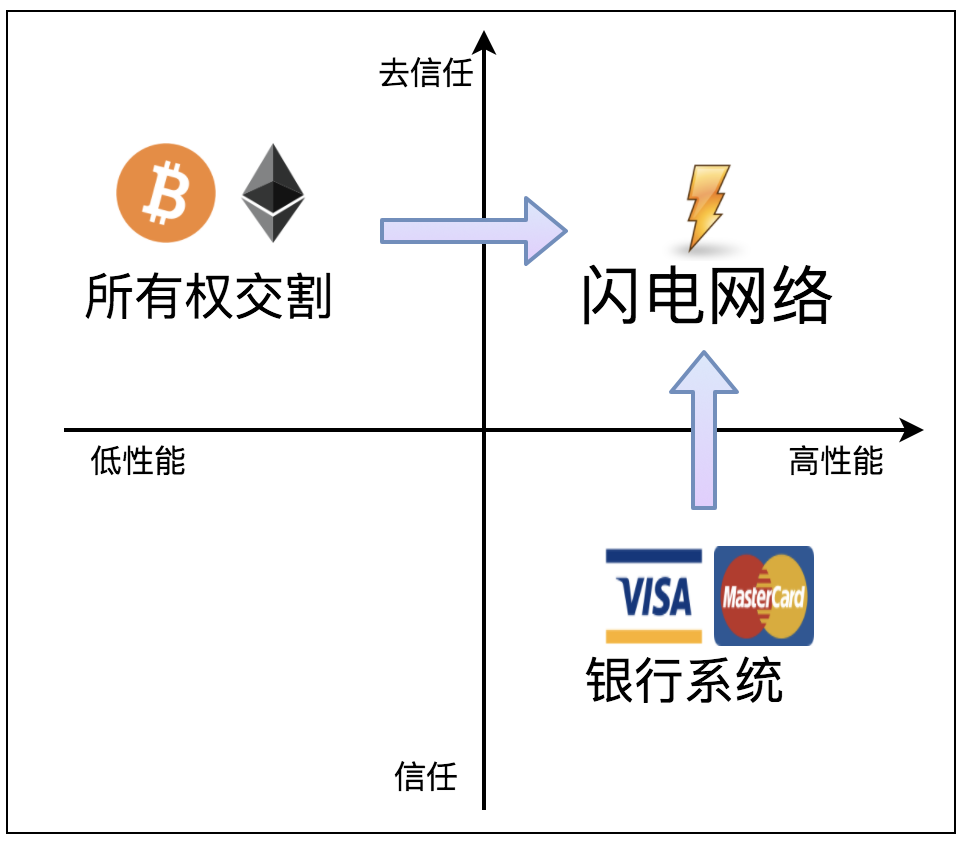
\includegraphics[width=8cm, keepaspectratio]{../images/comparision_1.png}
    \caption{分布式账本 vs. 清算中心}
    \label{fig:comparition}
\end{figure}


二者像是两个极端,互不相容。能否存在一种解决方案将银行系统和区块链的二者优点整合在一起呢?既能支持海量的支付场景,同时又不依赖于中介的信用?这个看似不可能完成的任务,闪电网络给我们提供了可行的解决方案。它是一种基于智能合约的去信任清算系统。

本章先阐述去信任清算的基本概念,可以帮助读者比较直观的理解闪电网络的思想和理念,有利于消化吸收下一章介绍的技术实现细节。

\subsection{基本概念}

\subsubsection{虚拟银行 Virtual Bank}
虚拟银行是运行于区块链上的一个智能合约,由支付双方共同协商创建。它模拟一个银行机构作为支付双方的公共债务人。虚拟银行部署之后,按照预先协商的额度,双方向虚拟银行的智能合约注入资金,完成虚拟银行的筹建。将来如果虚拟银行被清盘结算,资金都返还给支付双方,那么虚拟银行的服务自行终结。

\begin{figure}[h!]
    \centering
    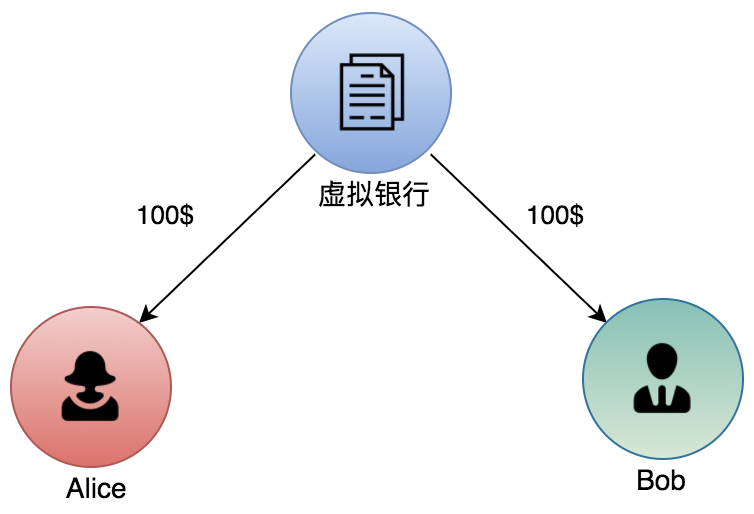
\includegraphics[width=8cm, keepaspectratio]{../images/channel.png}
    \caption{虚拟银行}
    \label{fig:virtualbank}
\end{figure}

和传统的银行相比,有三个特点:

\begin{itemize}
\item  \textbf{微型}: 一个虚拟银行只有两个账户,只管理特定交易双方的资产。所以资产负债表也只有2条数据。
\item  \textbf{无需信任}:虚拟银行是通过智能合约实现的,继承了智能合约的公开、透明、不可篡改、不可伪造、不可撤销等特点。所以作为公共债务人,虚拟银行没有传统金融机构的风险:比如对手风险、道德风险、流动性风险等。虚拟银行筹建完成之后,它的债务偿付能力永远是100\%,自然也不没有金融监管的成本。提供了无需信任的资产托管服务。
\item  \textbf{双重签名}:和一般银行的运营模式不同,虚拟银行不接受客户单方面取款请求。银行只有两个账户,而且总资产不变。一方的资产增加,意味着另一方的资产减少,这是一个零和博弈。为了防止单方面作弊行为,侵害对方的权益,虚拟银行智能合约在处理资产调整请求的时候,要验证双方的签名,保证每一次资产调整都是双方共同的真实意愿。
\end{itemize}


\subsubsection{共同承诺 (Mutual Commitment)}
每一次微支付,虚拟银行中的资产负债表要做一次调整。双方在链下对债务调整方案达成一致,形成向虚拟银行智能合约的请求消息,并且双方签名。此消息并不立刻广播到链上,而是由双方存储在本地,称之为\textbf{共同承诺}。共同承诺是双方真实意愿的表达,是彼此之间对资产分配方案的承诺。共同承诺一旦达成,在任何时候、任何一方都可以将承诺方案广播到链上,虚拟银行都会兑现承诺,按照预定方案结算银行的资产,分配到双方的账户中。共同承诺的作用类似于银行支票,虽然没有兑现,但是持有共同承诺就可以无风险的、随时的从虚拟银行中兑现响应的资产。

共同承诺的实现必须满足以下几个要求:

\begin{enumerate}
    \item \textbf{不可伪造}:共同承诺表达虚拟银行双方当事人的真实意愿,任何第三方无法伪造当事人的身份,生成虚假共同承诺。
    \item \textbf{不可篡改}:对于已经达成的承诺,其中的所有条款无法篡改。虚拟银行智能合约会检查双方的签名,确保承诺的完整性。
    \item \textbf{可以撤销}:共同承诺只要没有提交到虚拟银行兑现,双方可以达成新的承诺,并且撤销旧的承诺。对于交易双方来讲,只有最后的一份共同承诺是有效的,之前达成的历史承诺都应该撤销。可撤销性是通过撤销锁机制实现的。
    \item \textbf{文义证券}:在共同承诺的条款限定条件下,虚拟银行必须能够随时的、无风险的、按照承诺约定的分配方案结算资产。或者说,共同承诺具有文义证券、无因证券的特点。
\end{enumerate}

通俗的来讲,共同承诺就像是双方共同签署的支票,虚拟银行可以在任何时候兑现这张支票。和通常的支票不同的是:它同时处置两个人的资产,而且是虚拟银行中所有的资产都安全兑现。也就是说,一旦兑现某一个承诺,虚拟银行随即关闭。

闪电网络协议中有两种承诺方案:RSMC 承诺与 HTLC 承诺。他们的区别我们后面会讲,但是都满足上述4个条件。

\subsubsection{承诺编号 Sequence}
在共同承诺兑现之前,双方可以达成多次共同承诺,撤销旧的承诺,建立新的承诺。这些承诺按照时间顺序编号,以 Sequence 表示。


\subsubsection{进攻方(Attacker) 与 防御方(Defender)}
如果一方将共同承诺广播到链上,主动向虚拟银行发起申请, 重新结算资产,此方称之为承诺方案的进攻方。被动的接受他人资产分配方案的一方,称之为防御方。

虚拟银行的资产清算,相当于瓜分银行的总资产,是一种零和博弈。假设双方都是理性的决策者,任何一方都不会做出于对方有利,于己方不利的决策。双方需要一种公平的机制管理共同承诺,规避对手风险,防止对方作弊。

在闪电网络的协议里,一个新的承诺方案先由防御方初审。如果防御方接受此承诺方案,就对此签名,然后发送给进攻方进行二审。进攻方持有多个防御方已初审的承诺方案,有权放弃对己方不利的方案。同时有权选择广播共同承诺的时间,当他觉得合适的时候,再加上自己的签名,广播到链上,向虚拟银行请求结算资产。虚拟银行智能合约检验双方的签名,根据共同承诺的条款,公开、透明的结算双方的资产。

\subsubsection{对偶承诺方案 Dual Commitment}
和现实中的支票不同,共同承诺都是一式两份,双方各持有一份。两份承诺编号一致、分配方案一致。但是攻守位置互换。比如说 Alice 持有的那一份,Alice 是进攻方,Bob 是防御方(Bob已经初审签名);反之,Bob 持有的那一份中,Bob 是进攻方,Alice 是防御方(Alice 已经初审签名)。这两份承诺方案是一对,互为对偶承诺方案,具有同等效力。虚拟银行可以接受任何一份,但是只能接受一份。一份承诺被兑现,另外一份立即作废。

这样设计的好处有两个:一是保持共同承诺的活性,避免单点故障造成的死锁。因为防御方只能被动等待进攻方向虚拟银行发起请求。假如进攻方故障,不能行使进攻方的职责,防御方可以翻转角色,使用对偶承诺方案,以进攻方的身份完成资产的结算。二是保持灵活性和对称性,任何一方都可以随时主动兑现共同承诺,降低对手风险。

\subsubsection{撤销锁 Revocation Lock}
为了标识一个共同承诺方案已经被撤销,闪电网络协议设计了撤销锁机制。在每一份承诺方案中,进攻方必须要放置一个撤销锁。不同的承诺编号、不同的承诺方案镜像有不同的撤销锁。如果一共有 N 对承诺方案,那么需要有 2N 个不同的撤销锁。

撤销锁由承诺方案的进攻方管理,它实际是一个随机账户地址,对应的私钥由进攻方保管。如果进攻方要撤销某一个承诺方案,他必须公开对应的撤销锁私钥。反过来说,如果防御方从进攻方拿到了一个撤销锁的私钥,那么他可以相信进攻方确实放弃了对应的承诺方案。 

一般来讲,从虚拟银行开始,一共有 N 对共同承诺方案,前面的 (N - 1) 对承诺方案已经被撤销,这些历史承诺方案的撤销锁私钥是公开的,每一方都会保留一份对方的\textbf{撤销锁私钥列表}。只有最后一对承诺方案是有效的,其撤销私钥还没有公开。

撤销锁的安全机制:当一个承诺方案提交给虚拟银行的时候,防御方可以查看此撤销锁的编号(Sequence)。如果防御方发现此承诺方案是已经被撤销的,那么从\textbf{撤销锁私钥列表}中,找到对应的私钥,并且生成签名作为凭证,向虚拟银行证明对应的承诺方案是已经被撤销的。虚拟银行将判定进攻方违约,对进攻方处以罚金。这种情况称之为“\textbf{破解撤销锁}”。所以如果进攻方是理性的,他就不会冒着撤销锁被破解的风险提交已经撤销的承诺方案。反之,提交未撤销的承诺方案是安全的,因为防御方不知道撤销锁私钥,也就无法破解撤销锁。

当双方创建一对新的承诺方案的时候,需要交换旧承诺方案的失效私钥,表示双方都只承认新的方案,放弃旧的方案。在承诺方案兑现之前,双方都要妥善保存对方的\textbf{撤销锁私钥列表},防止对方使用对己方不利的承诺提案结算虚拟银行中的资产。

\subsubsection{诚信保证金 Fidelity Bond}
为了保证承诺方案的公平性,承诺方案会设立\textbf{诚信保证金}条款,和撤销锁机制配合使用。当虚拟银行兑现一份承诺方案的时候,防御方被动接受进攻方的资产分配方案,所以防御方的资产份额可以优先结算。而进攻方的所有资产作为\textbf{诚信保证金}冻结一段时间。目的是防止进攻方提交一份已经被撤销的承诺方案,侵犯防御方的利益。这个时间段成为\textbf{冻结期 Freeze Time}

在\textbf{诚信保证金}的冻结期间内,虚拟银行会等待防御方破解该方案的撤销锁。如果破解成功,防御方可以取走所有的诚信保证金作为惩罚。进攻方就会损失所有资产。反之,冻结期满之后,进攻方可以取走诚信保证金。

\subsubsection{支付通道}
支付双方以虚拟银行托管双方的资产,通过 RSMC 共同承诺重新清算双方的存款余额,已达到价值转移的效果,这种支付工具称之为支付通道。虚拟银行筹建并且达成初始 RSMC 共同承诺,标志着支付通道的开启;虚拟银行根据任何一方提交的承诺方案结算双方的资产,就标志着支付通道关闭。

\subsubsection{支付通道内在的信任机制}
在承诺方案的决策过程中,首先是防御方对承诺方案签名,拥有\textbf{初审权},可以拒绝对防御方不利的条款;然后进攻方对承诺方案签名,拥有\textbf{复审权},可以放弃对于进攻方不利的方案。二者的权利是对等的。

在承诺方案的执行过程中,进攻方拥有\textbf{提交权},有权选择什么时候提交、提交哪一个承诺方案;防御方拥有\textbf{监督权},有权检查承诺方案的有效性,挑战撤销锁,惩罚进攻方的违约行为;虚拟银行智能合约拥有\textbf{执行权},公开、公平的按照承诺方案的条款处置双方的资产。三者的权利是不同的,既互相独立、又互相制约。

\begin{figure}[h!]
    \centering
    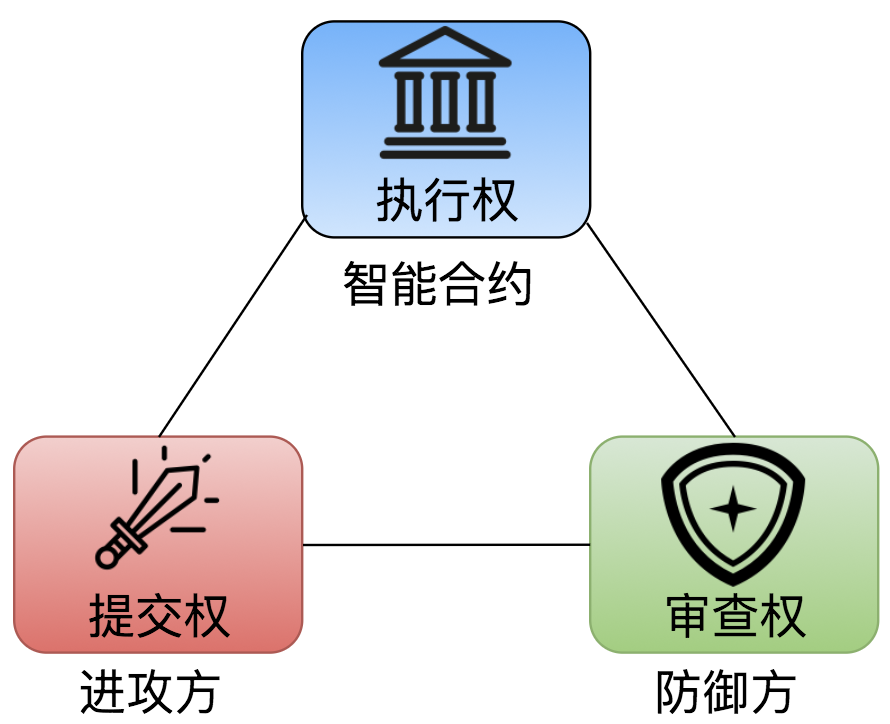
\includegraphics[width=6cm, keepaspectratio]{../images/trias.png}
    \caption{三权分立}
    \label{fig:trias}
\end{figure}

无论是决策阶段、还是执行阶段,基于虚拟银行智能合约的共同承诺协议,构建了一种均衡的二元博弈体系。此博弈的纳什均衡点,形成一种内生的信任机制,不需要外部的第三方监管与信用保障。就像有“一只看不见的手”,自动促使双方必须诚实的遵守共同承诺。

\subsection{RSMC承诺方案与支付通道}
在闪电网络中定义了两种承诺方案。第一种称为 RSMC(Recoverable Sequence Maturity Contract)承诺方案,定义了最基本的承诺方案,其中包括承诺编号、撤销锁、诚信保证金、对偶承诺方案等。

假设 Alice 和 Bob 创建了一个虚拟银行,上方初始的资产为 [100, 100]。双方的第一份共同承诺的方案如下图所示。
\begin{figure}[h!]
    \centering
    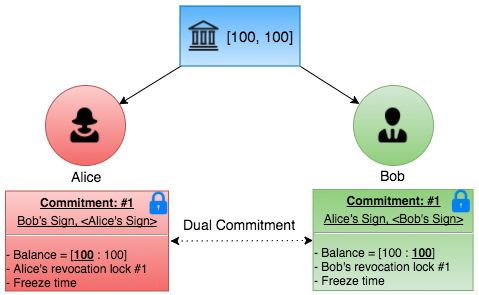
\includegraphics[width=8cm, keepaspectratio]{../images/rsmc_1.png}
    \caption{对偶 RSMC 承诺方案}
    \label{fig:rsmc_1}
\end{figure}

首先,承诺的 Header 部分有两部分:
\begin{itemize}
    \item \textbf{承诺编号}:此例中为 \#1。如 所述,每一个编号的承诺都是一式两份,分别为 Alice 和 Bob 持有。这两份承诺互为对偶承诺,攻守位置互换。左面Alice 持有的承诺是以 Alice 为进攻方,Bob 为防御方;反之,右面 Bob 持有的承诺以 Bob 为进攻方,Alice 为防御方。
    \item \textbf{双方的签名}:防御方作为初审,已经在承诺里面签名。进攻方的签名暂时还空着。比如说左面 Alice 的承诺中有 Bob 的签名"Bob's Sign",Alice 还未签名,用"<Alice's Sign>"表示。
\end{itemize}

在承诺的Body中,一共有三项:

\begin{itemize}
    \item \textbf{资产分配方案}:双方约定如何分配虚拟银行的资产,因为这一第一份方案,所以和双方的注资额度是一样的,也是[100, 100]。其中进攻方一方的资产(下划线标识)作为诚信保证金将会被锁定一段时间。
    \item \textbf{进攻方的撤销锁}: 由进攻方设定的撤销锁,对应的私钥由进攻方管理。如果此方案撤销,进攻方要公开撤销锁的私钥。
    \item \textbf{锁定期}:诚信保证金的锁定时间,此时间要足够长,使得防御方有足够的时间审查进攻方提交的承诺方案。
\end{itemize}


如果 Alice 向 Bob 支付 10 美元,双方会创建一个新的 RSMC 承诺方案,编号为 \#2, 而且分配方案改为:[90, 110]。如下图所示。除此之外,双方互相公开编号为 \#1 的承诺方案的撤销锁私钥,在新的承诺方案里换了新的撤销锁。

\begin{figure}[h!]
    \centering
    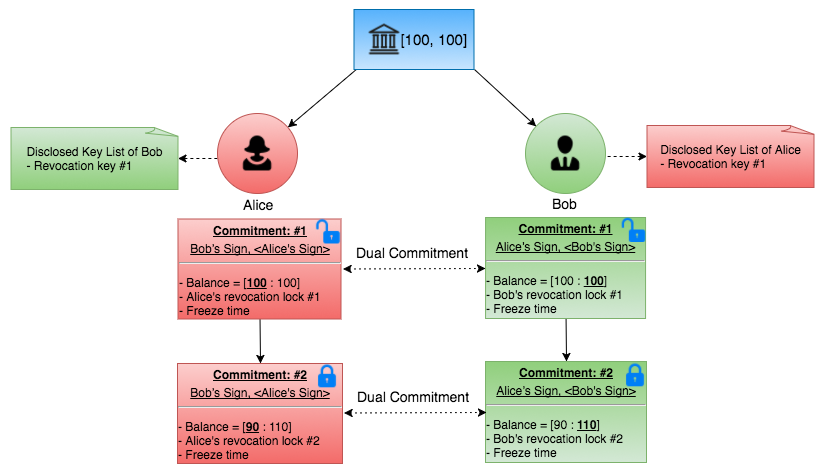
\includegraphics[width=16cm, keepaspectratio]{../images/rsmc_2.png}
    \caption{更新RSMC 承诺方案}
    \label{fig:rsmc_2}
\end{figure}

RSMC 承诺方案的特点是没有时间期限,只要没有被撤销,承诺永久有效。任何一方随时可以向虚拟银行提交 RSMC 承诺方案。

\subsection{HTLC承诺方案与支付通道网络}

\subsubsection{HTLC 承诺方案}
RSMC 协议的局限性在于虚拟银行自有两个账户,只能服务于两个人之间的往来支付。支付双方必须建立直连的支付通道,如果在N个人之间建立支付通道,那么每个人需要管理$(N-1)$个支付通道,总计一共有$(N - 1)*N/2$ 个支付通道。闪电网络进一步提出了 HTLC (Hashed Timelock Contract) 承诺方案,可以将支付通道的负责度从$O(N^2)$ 降低到 $O(N)$。

和 RSMC 一样,HTLC 中的承诺方案同样也具有不可伪造性、不可篡改性、可撤销性。这两种承诺方案的差异在于:HTLC 承诺方案除了撤销锁之外,还额外添加了时间锁和 Hash 锁条款。具体的来说:

\begin{itemize}
    \item \textbf{时间锁}:承诺只在规定时间内有效。
    \item \textbf{Hash锁}:支付的发送方向接收方出示一个 Hash 值 H,接收方必须公开对应的暗语R,使得 Hash( R ) = H。
\end{itemize}

接收方当且仅当满足这两个条件,就能获得约定的款项。否则将回退到上一个承诺方案的状态。

举个例子,如下图所示。假设根据当前的共同承诺编号为 \#2,余额是 [90美元, 110美元]。Alice 向 Bob 支付10美元。他们约定使用 HTLC 承诺方案,Bob 先生成一个随机数 R,计算其Hash值:H = hash(R),然后将 H 分享给 Alice,而且约定时间锁 T。那么HTLC 承诺方案的条款应该是这样的:

\begin{figure}[h!]
    \centering
    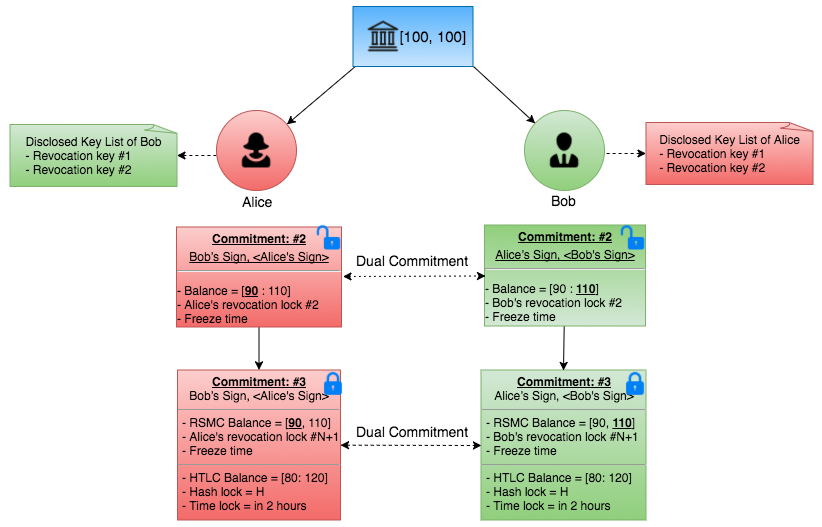
\includegraphics[width=16cm, keepaspectratio]{../images/htlc-1.png}
    \caption{HTLC 承诺方案}
    \label{fig:htlc}
\end{figure}
\begin{enumerate}
    \item 如果在时间 T 之前,任何一方提交承诺方案,检查暗语 R 是否符合 Hash 锁
        \begin{itemize}
            \item 如果符合,那么按照[80美元,120美元]的方案结算 Alice 和 Bob 的资产
            \item 如果不符合,那么此次承诺方案提交无效。
        \end{itemize}
    \item 如果在时间 T 之后,任何一方提交承诺方案,那么按照[90美元, 110美元]的方案结算 Alice 和 Bob 的资产。
\end{enumerate}


HTLC 承诺方案也是分为 Header 和 Body 两部分,其中 Header 部分和 RSMC 是一样的。只是在 Body 部分有差异。其中 Body 分为两部分。第一部分是RSMC 是一样的,表示如果超过了时间锁的期限,那么按照原来的 [90, 110] 方式分配资产。第二部分包含 Hash 锁和时间锁参数,以及新的资产分配方式 [80, 120],如果满足了 Hash 锁与时间锁的要求,就按照新的方式分配资产。

当 \#3 号承诺方案达成的时候,双方公开 \#2 号承诺方案的撤销锁私钥,表示放弃旧的承诺方案。相对于 RSMC 来说,HTLC 承诺方案是带有限制性条件的临时承诺方案。

\subsubsection{支付路径}
HTLC 承诺方案的价值在于可以将首尾相连的多个支付通道串联起来,建立支付路径。如图所示,Alice 和 Carol 没有直接关联的支付通道,但是他们分别与 Bob 建立了支付通道。那么 Alice - Bob - Carol 形成了一条支付路径,他们可以通过支付路径也可以完成支付。假设Alice 向 Carol 支付10美元,基本过程如下:

\begin{figure}[h!]
    \centering
    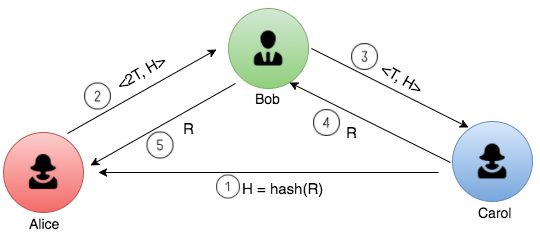
\includegraphics[width=8cm, keepaspectratio]{../images/payment_path.png}
    \caption{支付路径}
    \label{fig:htlc_path}
\end{figure}

\begin{enumerate}
    \item Carol 随机产生暗语 R,计算Hash 值: H = hash(R),并将 H 发送给 Alice。
    \item Alice 和 Bob 达成 HTLC 承诺:如果Bob能在时间 \textbf{2T} 内出示暗语 R,使得 hash(R) = H, 那么Alice 向 Bob 支付 10 美元。
    \item Bob 再和 Carol 达成 HTLC 承诺:如果 Carol 能在更短的时间 \textbf{T} 内出示暗语 R,使得 hash(R) = H, 那么Bob 向 Carol 支付 10 美元。
    \item 由于 Carol 知道暗语 R 值,在规定的期限T内,可以把R出示给 Bob,获得 Bob 的10美元。之后 Bob 和 Carol 可以再签署一份 RSMC 承诺方案,代替临时的 HTLC 承诺方案。
    \item Bob 从 Carol 那里拿到暗语 R 的时候,和 Alice 之间的 HTLC 承诺还没有过期,向 Alice 出示 R 之后,可以获得 10 美元。然后也可以再重新签署一份无期限的 RSMC 承诺,替换临时的 HTLC 承诺方案。
\end{enumerate}

最终的结果就是:Alice 通过 Bob 向 Carol 支付了 10美元,Bob 作为中间人资产并没有变化。HTLC 承诺方案可以在两个联通的支付通道上传递交易,整个过程是可信的。我们从支付通道内和支付通道间两个方面考察对手风险问题。

\subsubsection{支付通道内的对手风险}
首先,支付的接收方无法伪造暗语 R 而欺诈对方,在规定的时间内破解 Hash 锁是不可能的。

其次,双方在达成 HTLC 共同承诺之后,可以安全的撤销原来的承诺方案。对于接收方来讲,及时公开暗语 R 值,就可以获得 10 美元,所以放弃原承诺方案没有风险。对于发送方来讲,如果没有及时公开暗语 R,那么就回退到原来的状态;如果及时公开暗语 R,他就可以从前面的一个支付通道获得 10 美元,总之也可以无风险的放弃原有的承诺方案。

再次,双方在达成 HTLC 共同承诺之后,发送方不需要担心接收方在获得 10 美元的情况下,不及时把暗语 R 发送给自己。否则接收方必须在规定时间内向虚拟银行提交HTLC 承诺方案,其中包含暗语 R。从智能合约的公开交易数据中,发送方依然可以获得暗语 R。

最后,公开暗语 R 之后,双方可以在时间锁 T 到期之前,按照新的资产负债表建立无时间期限的 RSMC 承诺方案,撤销临时的 HTLC 承诺方案。接收方无疑不会反对替换新承诺方案;对于发送方来讲,拒绝替换方案也没有意义,因为如果发送方想拖延时间,等时间锁过期之后,HTLC 承诺回退,那么接受方为了保护自己的利益,可以及时提交 HTLC 承诺方案,兑现属于自己的10美元。发送方不但无法取回10美元,而且需要重新建立支付通道。

\subsubsection{支付通道间的对手风险}

注意到 HTLC 承诺方案是沿着支付路径,从发送方向接收方建立;然后暗语是反方向,从接收方向发送方传递。对于任何一个中间节点,必须向接收端一侧支付 10 美元才能知道暗语 R,否则无法从发送端一侧获得 10 美元的补偿。另一方面,由于发送端的时间锁比接受端的长,当他拿到暗语 R 之后,也有充足的时间,可以无风险的获得 10 美元。

对于更长的支付路径,HTLC 承诺方案依然有效。需要注意的是,资金从接收方向发送方传播,每经过一段支付通道,对应的时间锁要增加一个 T,保证资金的发送方有足够的时间向接收到下一个发送方的资金。进一步推广,所有的支付通道链接在一起构成了\textbf{支付通道网络},其中某一些特定的节点作为中心枢纽,链接其它普通节点。一个节点要向另一个节点支付,只要找到一条联通二者的路径,而且路径上的每一段都都有充足的额度,就可以通过这条路径完成价值转移到过程。



